\documentclass{article}
\usepackage{fancyhdr}
\usepackage{extramarks}
\usepackage{amsmath}
\usepackage{amsthm}
\usepackage{amsfonts}
\usepackage{tikz}
\usepackage[plain]{algorithm}
\usepackage{algpseudocode}

\begin{document}
\author{Chuan Lu}
\title{PHYS:5905 Homework 3}
\maketitle

\medskip

\begin{enumerate}

\item
Third order Adams-Bashforth timestepping.

\begin{enumerate}
\item
I choose the last initialization method: 1 Euler with 4 leapfrog steps.

\item
Figure \ref{problem 1.2} is the error plot with respect to the number of timesteps. The slope is $k = -3.0021$.
\begin{figure}[h]
\centering
\vbox{
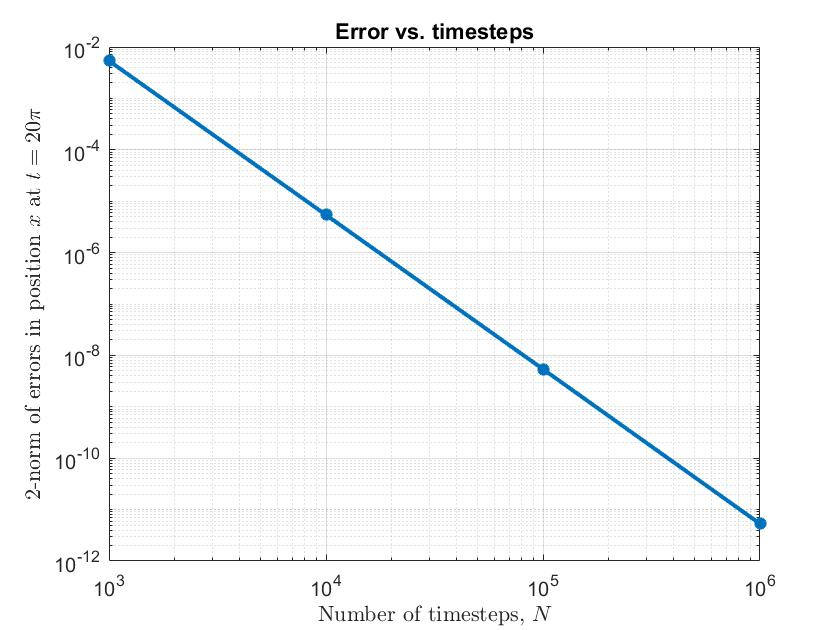
\includegraphics[scale=0.4]{problem1/error.jpg}
}
\caption{The error at $t = 20\pi$ with respect to the number of timesteps $N$.}
\label{problem 1.2}
\end{figure}

\end{enumerate}

\item
$\nabla B$ drift.

\begin{enumerate}
\item
Figure \ref{problem 2.1} shows the trajectory on the $(x, y)$ plane. 
\begin{figure}[h]
\centering
\vbox{
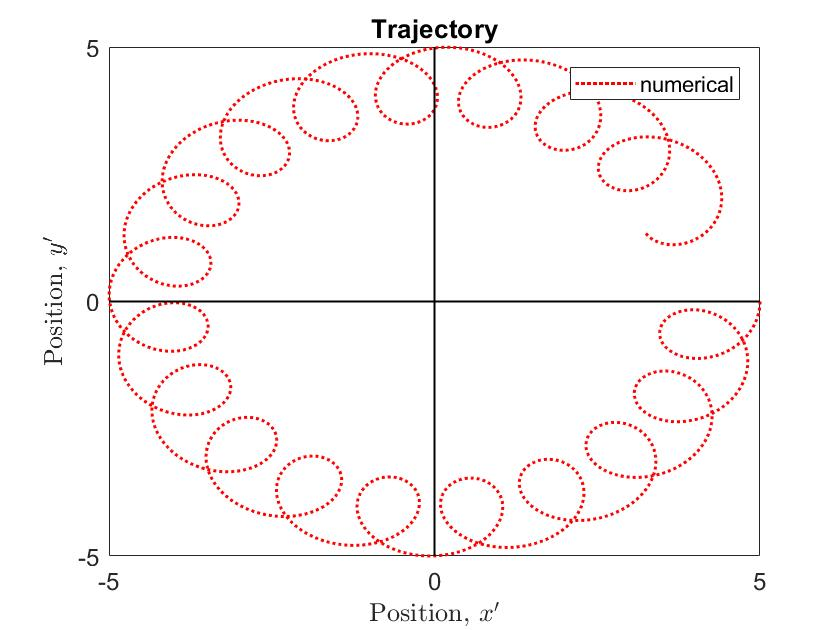
\includegraphics[scale=0.4]{problem2/trajectory.jpg}
}
\caption{The trajectory in the $(x, y)$ plane with AB3 scheme and $N=1000$ timesteps, and final time $T' = 30\pi$.}
\label{problem 2.1}
\end{figure}

\item
From Fig \ref{problem 2.2}, the minimum number of timesteps $N = 5000$.
\begin{figure}[h]
\centering
\vbox{
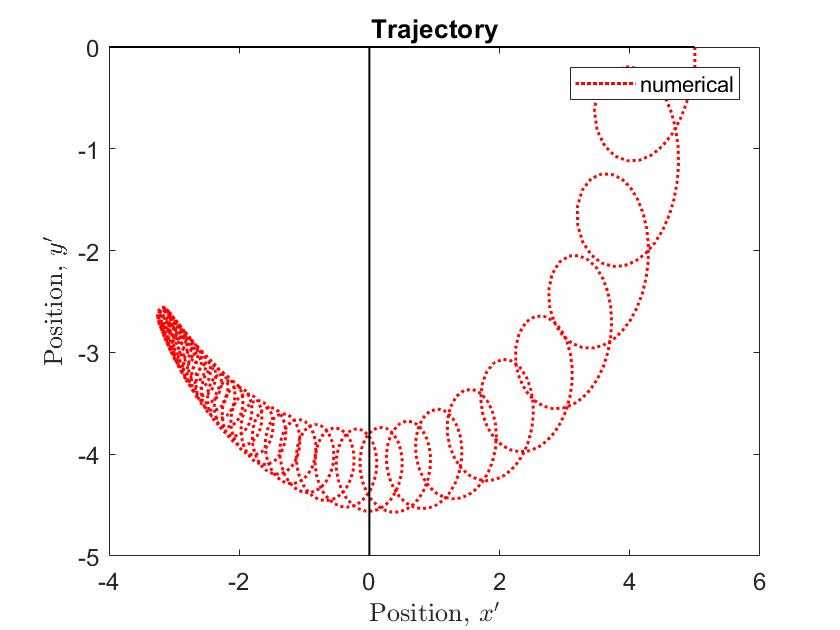
\includegraphics[scale=0.2]{problem2/1000.jpg}
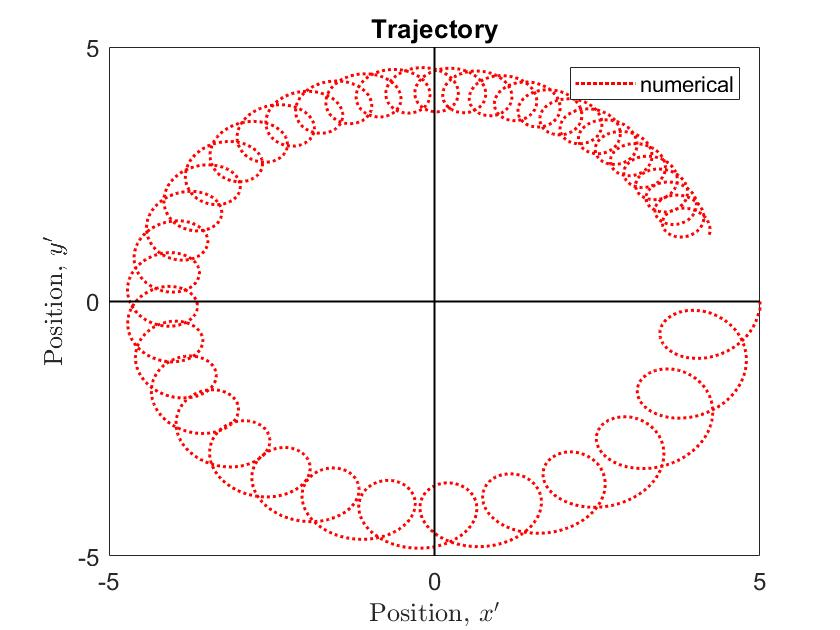
\includegraphics[scale=0.2]{problem2/1500.jpg}
}
\vbox{
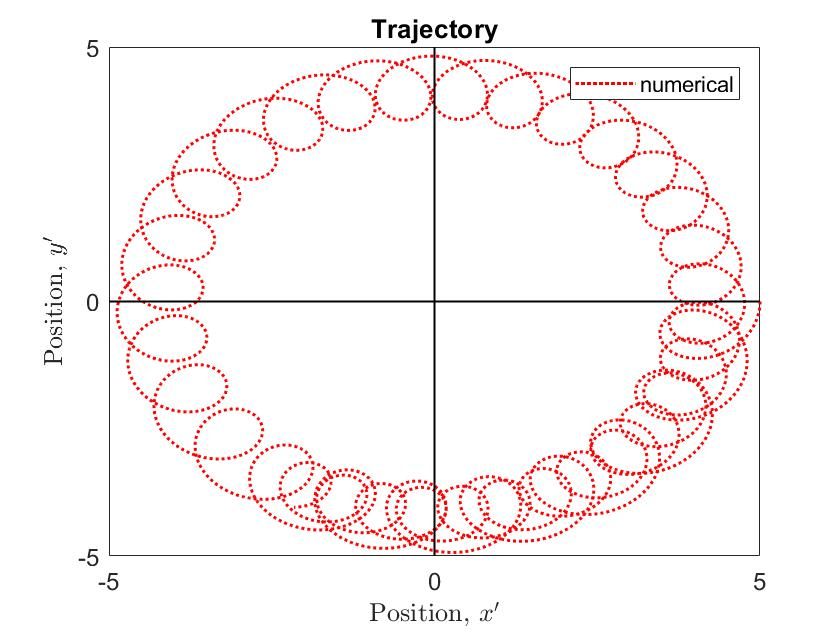
\includegraphics[scale=0.2]{problem2/2000.jpg}
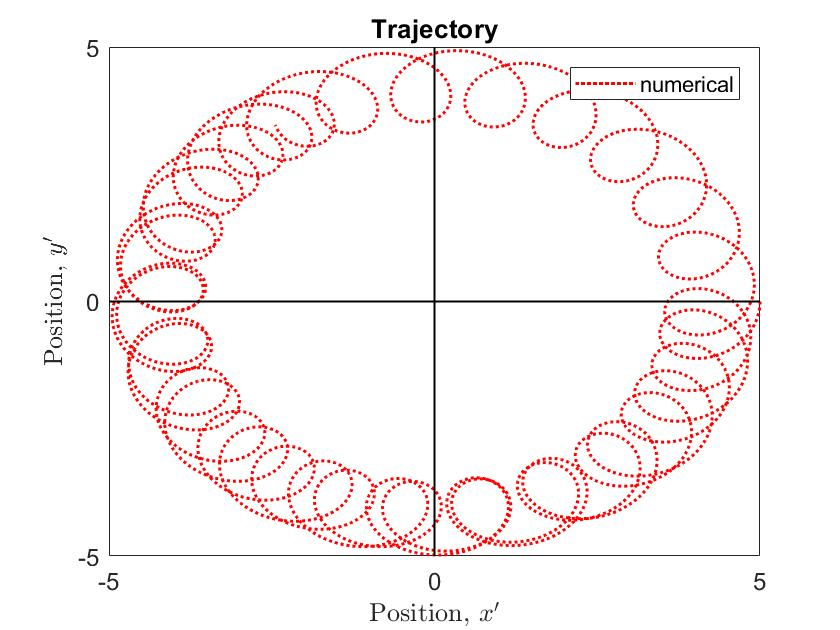
\includegraphics[scale=0.2]{problem2/3000.jpg}
}
\vbox{
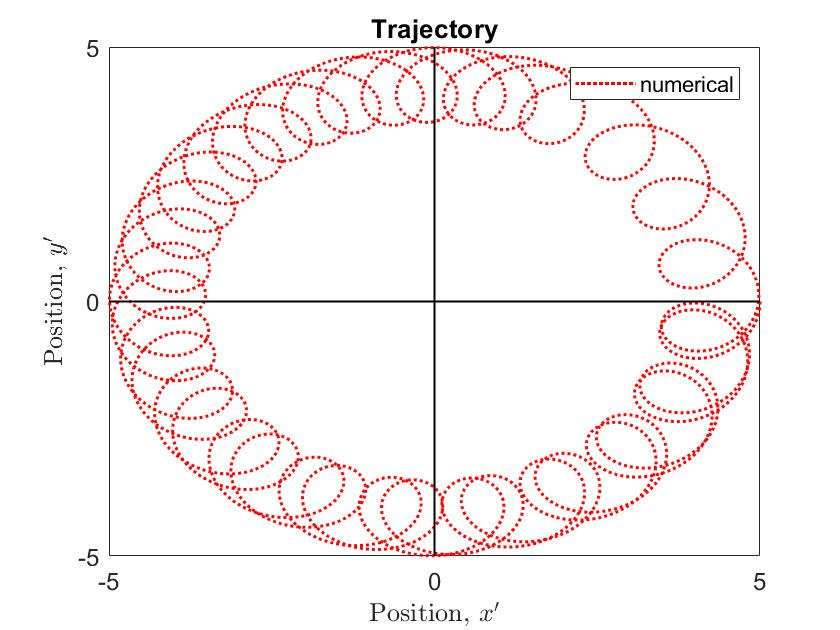
\includegraphics[scale=0.4]{problem2/5000.jpg}
}
\caption{The trajectory in the $(x, y)$ plane with AB3 scheme. Top: $N=1000, 1500$. Middle: $N=2000, 3000$. Bottom: $N=5000$}
\label{problem 2.2}
\end{figure}

\item
One possible way to check the numerical method is to increase the number of timesteps and see if the numerical results are consistent, and at the same time check if the solution is consistent with the physical model.

\end{enumerate}

\item Ring Current due to $\nabla B$ Drift


\item $\nabla B$ and Curvature Drifts

The trajectory is shown in Figure \ref{problem 4}.
\begin{figure}[h]
\centering
\vbox{
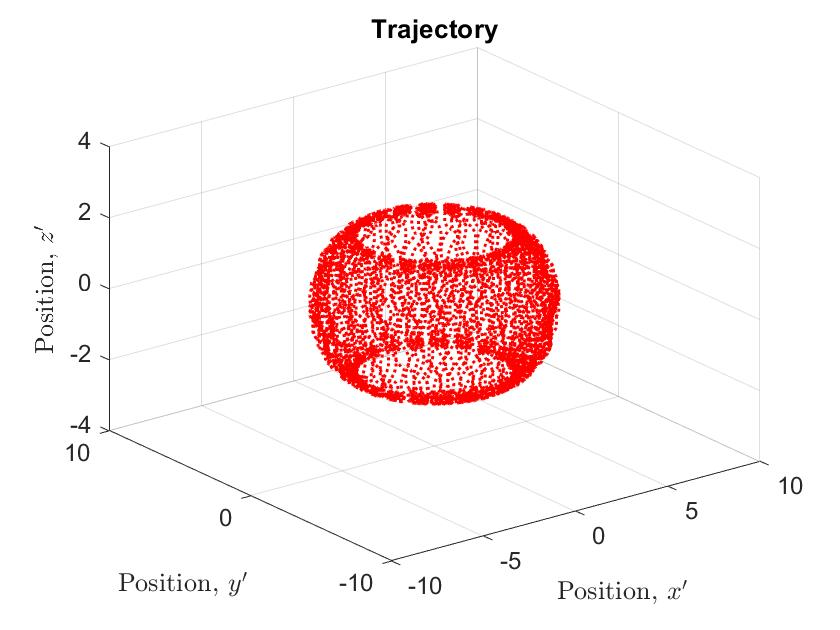
\includegraphics[scale=0.4]{problem4/trajectory.jpg}
}
\caption{The trajectory in the $(x, y, z)$ plane with AB3 scheme and $N=10^6 $ timesteps.}
\label{problem 4}
\end{figure}




\end{enumerate}


\end{document}